\documentclass[conference]{IEEEtran}
\IEEEoverridecommandlockouts
\usepackage{cite}
\usepackage{amsmath,amssymb,amsfonts}
\usepackage{algorithmic}
\usepackage{graphicx}
\usepackage{textcomp}
\usepackage{xcolor}
\usepackage{booktabs}
\def\BibTeX{{\rm B\kern-.05em{\sc i\kern-.025em b}\kern-.08em
    T\kern-.1667em\lower.7ex\hbox{E}\kern-.125emX}}


\begin{document}

\title{Policy-Guided Schema-Aware Framework for Semi-Structured Document Information Extraction}

\author{
\IEEEauthorblockN{Ayush Kumar}
\IEEEauthorblockA{\textit{School of Computer Science and Engineering (SCOPE)} \\
\textit{Vellore Institute of Technology}\\
Vellore, India \\
ayush.kumar2022a@vitstudent.ac.in}
\and
\IEEEauthorblockN{Ramesh C}
\IEEEauthorblockA{\textit{School of Computer Science and Engineering (SCOPE)} \\
\textit{Vellore Institute of Technology}\\
Vellore, India \\
ramesh.chandran@vit.ac.in}
}

\maketitle

% -----------------------------------------------------------------------
%  ABSTRACT
% -----------------------------------------------------------------------
\begin{abstract}
This work proposes a policy-guided schema-aware information extraction system for semi-structured documents, by integrating an OCR-free Donut branch with a layout-aware LayoutLMv3-based extraction branch. These two models are fused at the field level using deterministic policy-guided fusion, scoring, normalization, and consistency enforcement across fields. We employ a schema registry for semantic retrieval of pre-defined schemas and LoRA adapters for parameter-efficient adaptation of the LayoutLMv3 backbone for a variety of document formats.
In addition, we incorporate mechanisms for OCR fallback, schema validation, and recovery.
We assess the performance of the LoRA adapters on heterogeneous document datasets, and provide a proof-of-concept end-to-end evaluation covering multiple document types. The empirical results illustrate the viability of complementary information extraction models through deterministic policy guided fusion in a unified document processing pipeline. Given the restricted scale of the end-to-end evaluation, additional validation using comprehensive benchmark datasets is required.
\end{abstract}

\begin{IEEEkeywords}
document information extraction, schema-aware extraction, LayoutLMv3, LoRA,
semi-structured documents, policy-guided fusion
\end{IEEEkeywords}

% -----------------------------------------------------------------------
%  I. INTRODUCTION
% -----------------------------------------------------------------------
\section{Introduction}

The increasing digital adoption of business processes generates vast amounts of semi-structured documents that need to be effectively analyzed. These documents typically contain natural language text as well as non-textual elements such as layout and column structure; hence, the position of specific fields within these documents can vary drastically between different versions, vendors, and countries. Consequently, attempting to extract information based on the position of such fields will not be viable.

Historically, process and rules-based methods were employed to extract the information from these documents. Such methods were replaced by layout-aware models like LayoutLM \cite{layoutlm}, LayoutLMv2 \cite{layoutlmv2}, and LayoutLMv3 \cite{layoutlmv3}; more recently, models like Donut \cite{kim2022donut} that do not require optical character recognition and are agnostic to the layout of the document have been introduced.

Furthermore, with the introduction of large language models (LLMs) \cite{gptner2024}, it is possible to automatically extract information from documents in a largely unsupervised manner. However, LLMs tend to generate unanchored outputs when extracting information from documents \cite{ji2023hallucination}. One way to address this problem is to incorporate machine learning models that utilize deterministic verification mechanisms. We propose a framework that simultaneously utilizes layout-aware and OCR-free models, as well as a field-level deterministic fusion module that utilizes information regarding each field’s availability, agreement, confidence, attributes, and dependencies to deterministically fuse field candidates.

In addition to incorporating both layout-aware and OCR-free models, we additionally incorporate schema retrieval and parameter-efficient (LoRA) adaptation of LayoutLMv3.

Our goal in building this framework is not to reveal the best way to extract information from documents; rather, we aim to investigate different models that can be combined within a pipeline to achieve such a goal.


% -----------------------------------------------------------------------
%  II. RELATED WORK
% -----------------------------------------------------------------------
\section{Related Work}
\label{sec:related}

Layout-aware models such as LayoutLM\cite{layoutlm}, LayoutLMv2\cite{layoutlmv2}, and LayoutLMv3\cite{layoutlmv3} extract text, spatial, and visual features well on datasets such as FUNSD\cite{jaume2019funsd}, CORD\cite{park2019cord}, and DocVQA; FormNet\cite{lee2022formnet} and Hwang et al.\cite{hwang2021cost} propose approaches that explicitly model form label-value structures and perform rule-based form field extraction, respectively.  Our layout-aware branch is based upon LayoutLMv3 but adapted using LoRA instead of fine-tuning.  Donut\cite{kim2022donut} performs OCR-free field extraction from document images using a Swin-Transformer and BART model architecture; we adopt this method as-is with the off-the-shelf model weights.  Finally, DocVQA\cite{mathew2021docvqa} has influenced the design of the questions we ask of our models.

Many prompting methods based on language models such as GPT-NER\cite{gptner2024} allow for the extraction of information from documents with little annotation cost; however, these methods tend to propose hallucinated outputs \cite{ji2023hallucination} that are problematic for many applications.  Approaches like CUAD\cite{cuad2021} and Binmakhashen and Mahmoud\cite{binmakhashen2020} find it difficult to extract information at the clause level or to handle layouts of fields within documents that differ across those documents.  Iterative agentic methods such as ReAct\cite{react2023}, Reflexion\cite{reflexion2023}, and Self-Refine\cite{selfrefine2023} propose iterative loops that allow language models to self-correct their generated outputs; however, our policy network takes a different architectural approach and only performs a single pass through the network to generate its extraction results.  Thus, while we do cite these methods for motivation, they are outside the scope of our work.  Methods that use graphs to represent the information to be extracted from natural language documents \cite{yu2021pick} provide another motivation for the way that spatial information is injected into the fusion layer.

LoRA\cite{hu2022lora} provides a means of adapting a language model using only a small fraction of the model’s parameters; He et al.\cite{he2022unified} have unified adapter networks, prefix tuning, and LoRA-style methods under a common framework.  While PEFT methods have been applied to various natural language tasks, the joint adaptation of layout-aware models across spatial, visual, and textual features remains underexplored.  Thus, we propose grouping the seven document understanding datasets into two groups adapted using the LoRA method.


% -----------------------------------------------------------------------
%  III. RESEARCH GAP AND PROBLEM FORMULATION
% -----------------------------------------------------------------------
\section{Research Gap and Problem Formulation}
\label{sec:gap}

\subsection{Research Gap}

Current document information extraction methods mostly focus on either single layout-aware or OCR-free models, and evaluate them against schema-specific tasks. However, deterministic reconciliation of various extractor outputs with an end-to-end pipeline incorporating schema retrieval, parameter efficient cross-domain adaptation and validation has yet to be studied thoroughly. 



\subsection{Problem Formulation}

Given a semi-structured PDF document, and a schema of typed fields along with their description and constraints, we must output field-value pairs which must satisfy the given constraints, are traceable to the original document, are produced deterministically, and have an associated confidence score in [0, 1]. The document may be native or scanned(with OCR on it), and the schema can either be pre-defined or retrieved on the fly from a schema registry.

% -----------------------------------------------------------------------
%  IV. SYSTEM ARCHITECTURE AND METHODOLOGY
% -----------------------------------------------------------------------
\section{System Architecture and Methodology}
\label{sec:arch}

\begin{figure}[htbp]
    \centering
    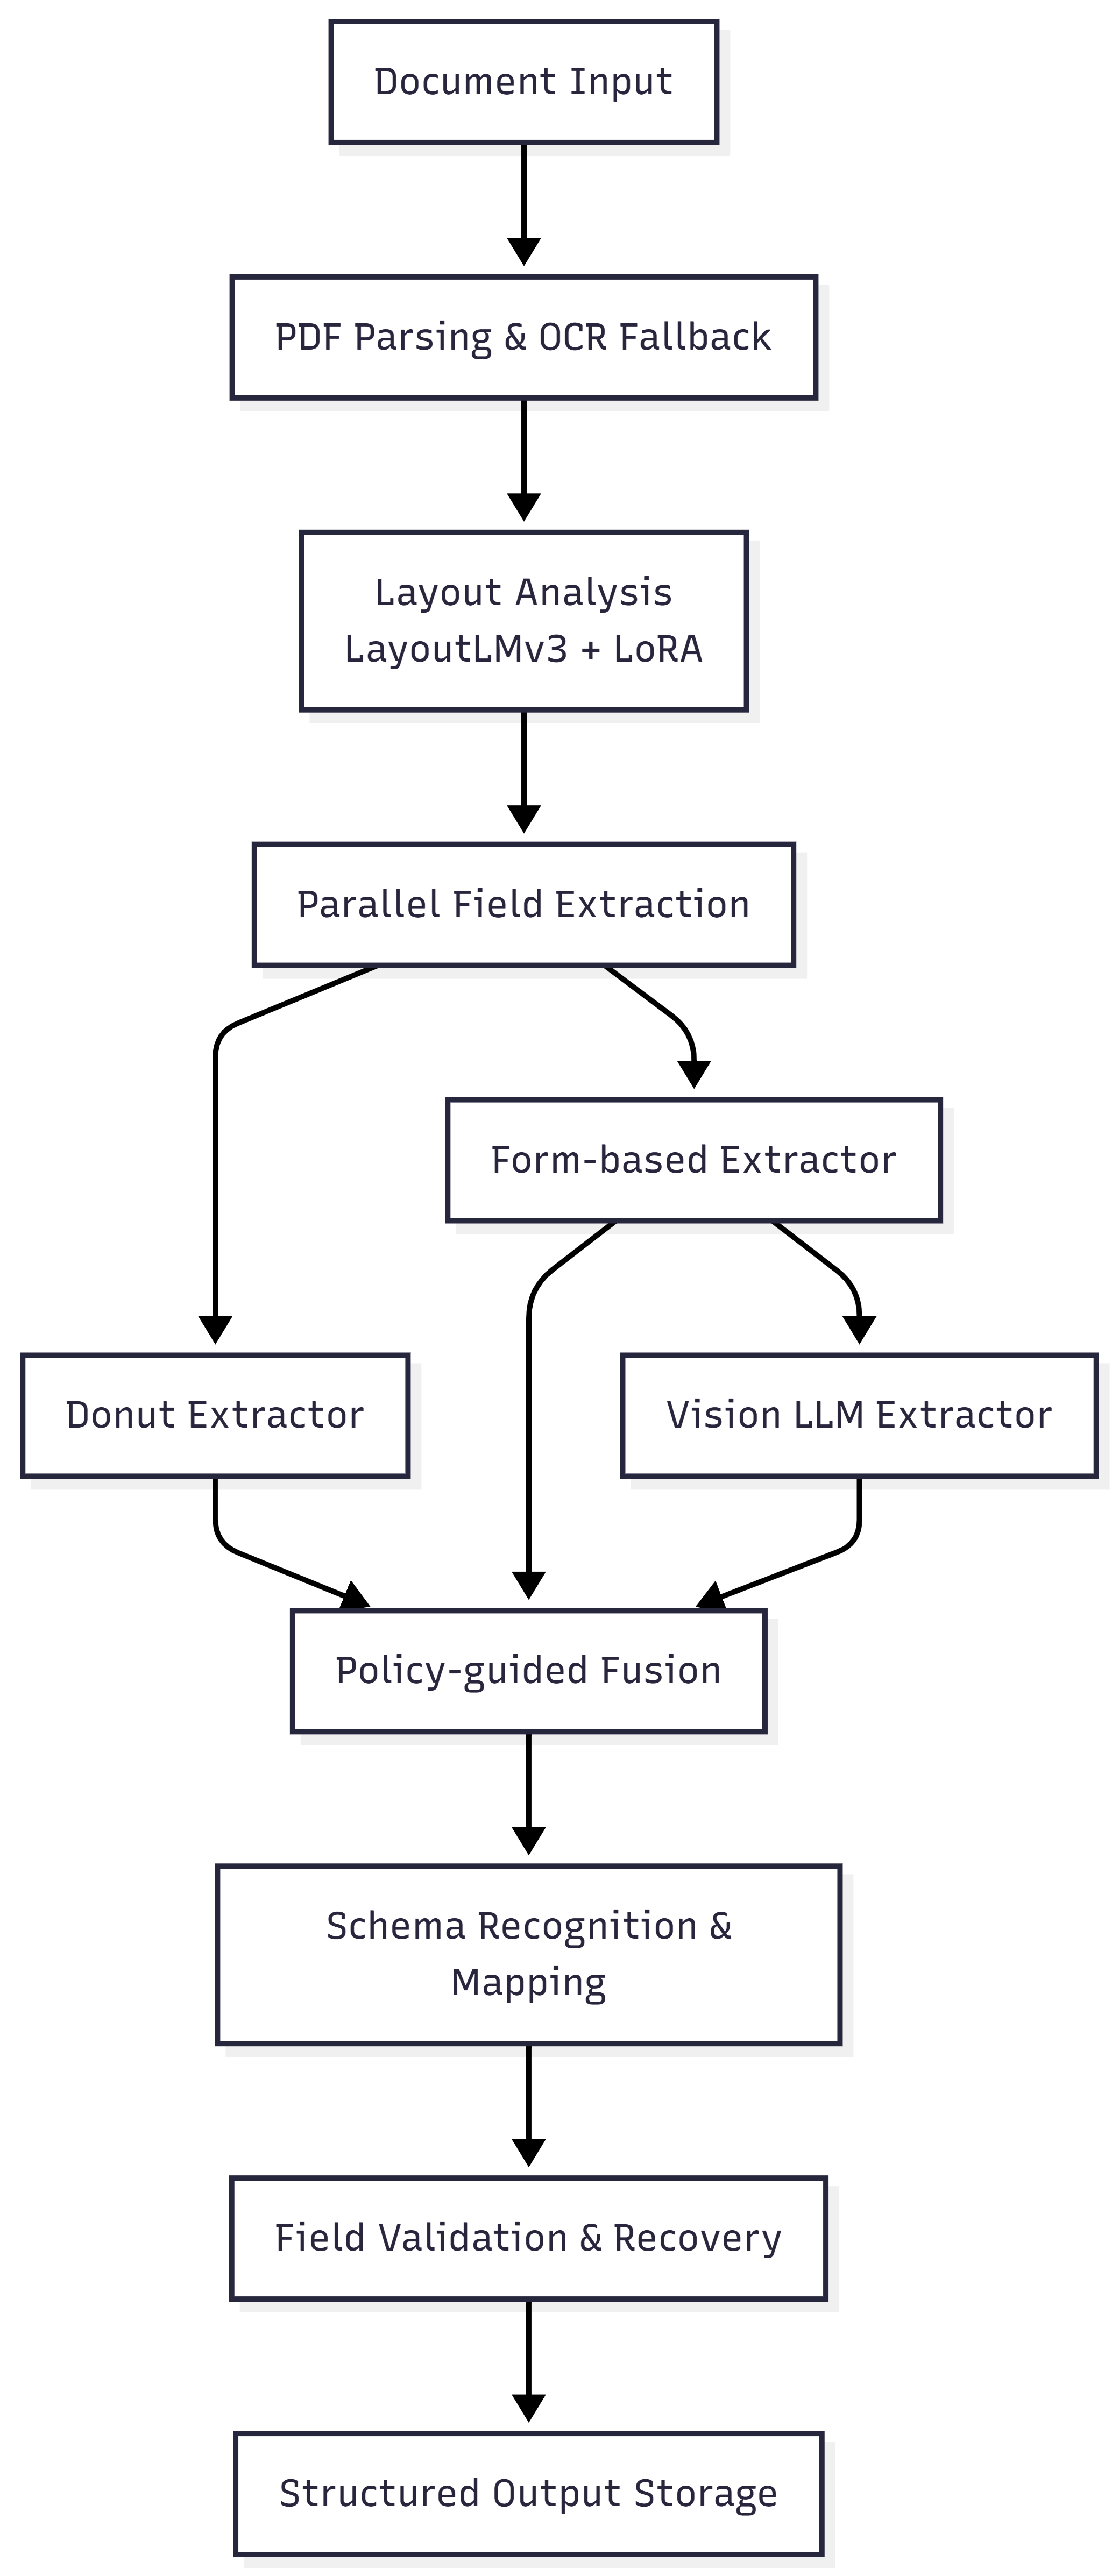
\includegraphics[width=0.6\columnwidth]{architecture.png}
    \caption{Architecture for the Proposed System}
    \label{fig:system_architecture}
\end{figure}

This pipeline has eight stages of extraction. Each stage passes a shared state from previous stage(s) to next (including any error it encounters), consisting of the blocks of documents being ingested, the image of the rendered page, the adapters that have been chosen for use, the results from the two extractors that were run to produce an extraction bundle, the fusion of policies applied to the output of the two extractors, the final resolved schema after all of the above steps are done, validation outcomes for each field after validation was run, a reference key for storing the data to be stored and any accumulated errors. The adapter group used to perform layout aware extraction is determined once before all of the extraction stages are run using the identified or retrieved schema name. Each stage will process exceptions independently. So if there is a problem in one stage then subsequent stages can continue with a partial state instead of failing completely.

\subsection{Document Ingestion with OCR Fallback}

The ingestion stage accepts PDF files as input, and produces a stream of document blocks. Each document block contains information about a single page in the PDF file, including a page number, all text that was found on the page, a bounding rectangle defined by four points $(x_0,y_0,x_1,y_1)$, a confidence value and a source tag describing how the text was obtained (either "native" or "ocr"). For digital PDFs, we attempt to get native text through PyMuPDF first. We consider native extraction insufficient for pages that contain less than 20 characters or five words. Pages that do not meet these criteria are rendered into images at a doubled horizontal and vertical scale factor ($2\times$). However, the scale factor is halved if $\max(\text{width},\text{height})>5000$ pixels in order to limit both memory usage and processing cost. In addition to other information contained within the OCR derived block, each block also includes an individual word level extraction confidence that is provided by Tesseract. This confidence is used later down-stream by the policy fusion layer.

\subsection{LoRA Adapter-Routed Layout Analysis}

\subsubsection{Dataset Grouping}

Seven datasets are split into two groups by adapter type, Group 1 (primitive layout extraction, including CORD, SROIE, and SynthDog-EN) and Group 2 (structural/layout classification, including FUNSD, RVL-CDIP, DocLayNet, and DocBank). Group 1 and Group 2 are fine-tuned separately on top of a frozen LayoutLMv3 base model with respective LoRA adapters. This grouping is done by data similarity, not based on an actual training schedule (i.e. Training a Group 2 adapter is independent from what the Group 1 adapter has learned).

\subsubsection{Adapter Setup}

A LoRA adapter for all Query, Key, Value, and Output projection layers in the LayoutLMv3 encoder are trained, with hyperparameter settings in Table \ref{tab:hyperparams}. A single adapter-router can maintain the frozen base model and keep a few recently-used adapters in memory, and can switch between groups of adapters by using PEFT commands \texttt{set\adapter} and \texttt{load\adapter}.

\subsubsection{Unifying Heterogeneous Label Spaces}

 Seven datasets have different levels of detail and native tasks (e.g., document-level classification for RVL-CDIP and word/region level layouts for other datasets). We thus first transfer native labels into a set of common coarse labels: header, body text, table, figure, and signature. Token-level labeling is achieved by including token centers in segments, instead of exact positional matching. For each OCR token (which consists of the OCR text and a bounding box normalized coordinates into [0,1000] and represented as $w = (x0^w, y0^w, x1^w, y1^w)$, we check for inclusion of the token's center point into annotated segments and assign the first containing segment as the token label, or use a background label if it is not inside any. This process can unify different supervisions in word-, region-, and document-level data.

\subsection{Parallel Extraction}

\begin{figure}[htbp]
    \centering
    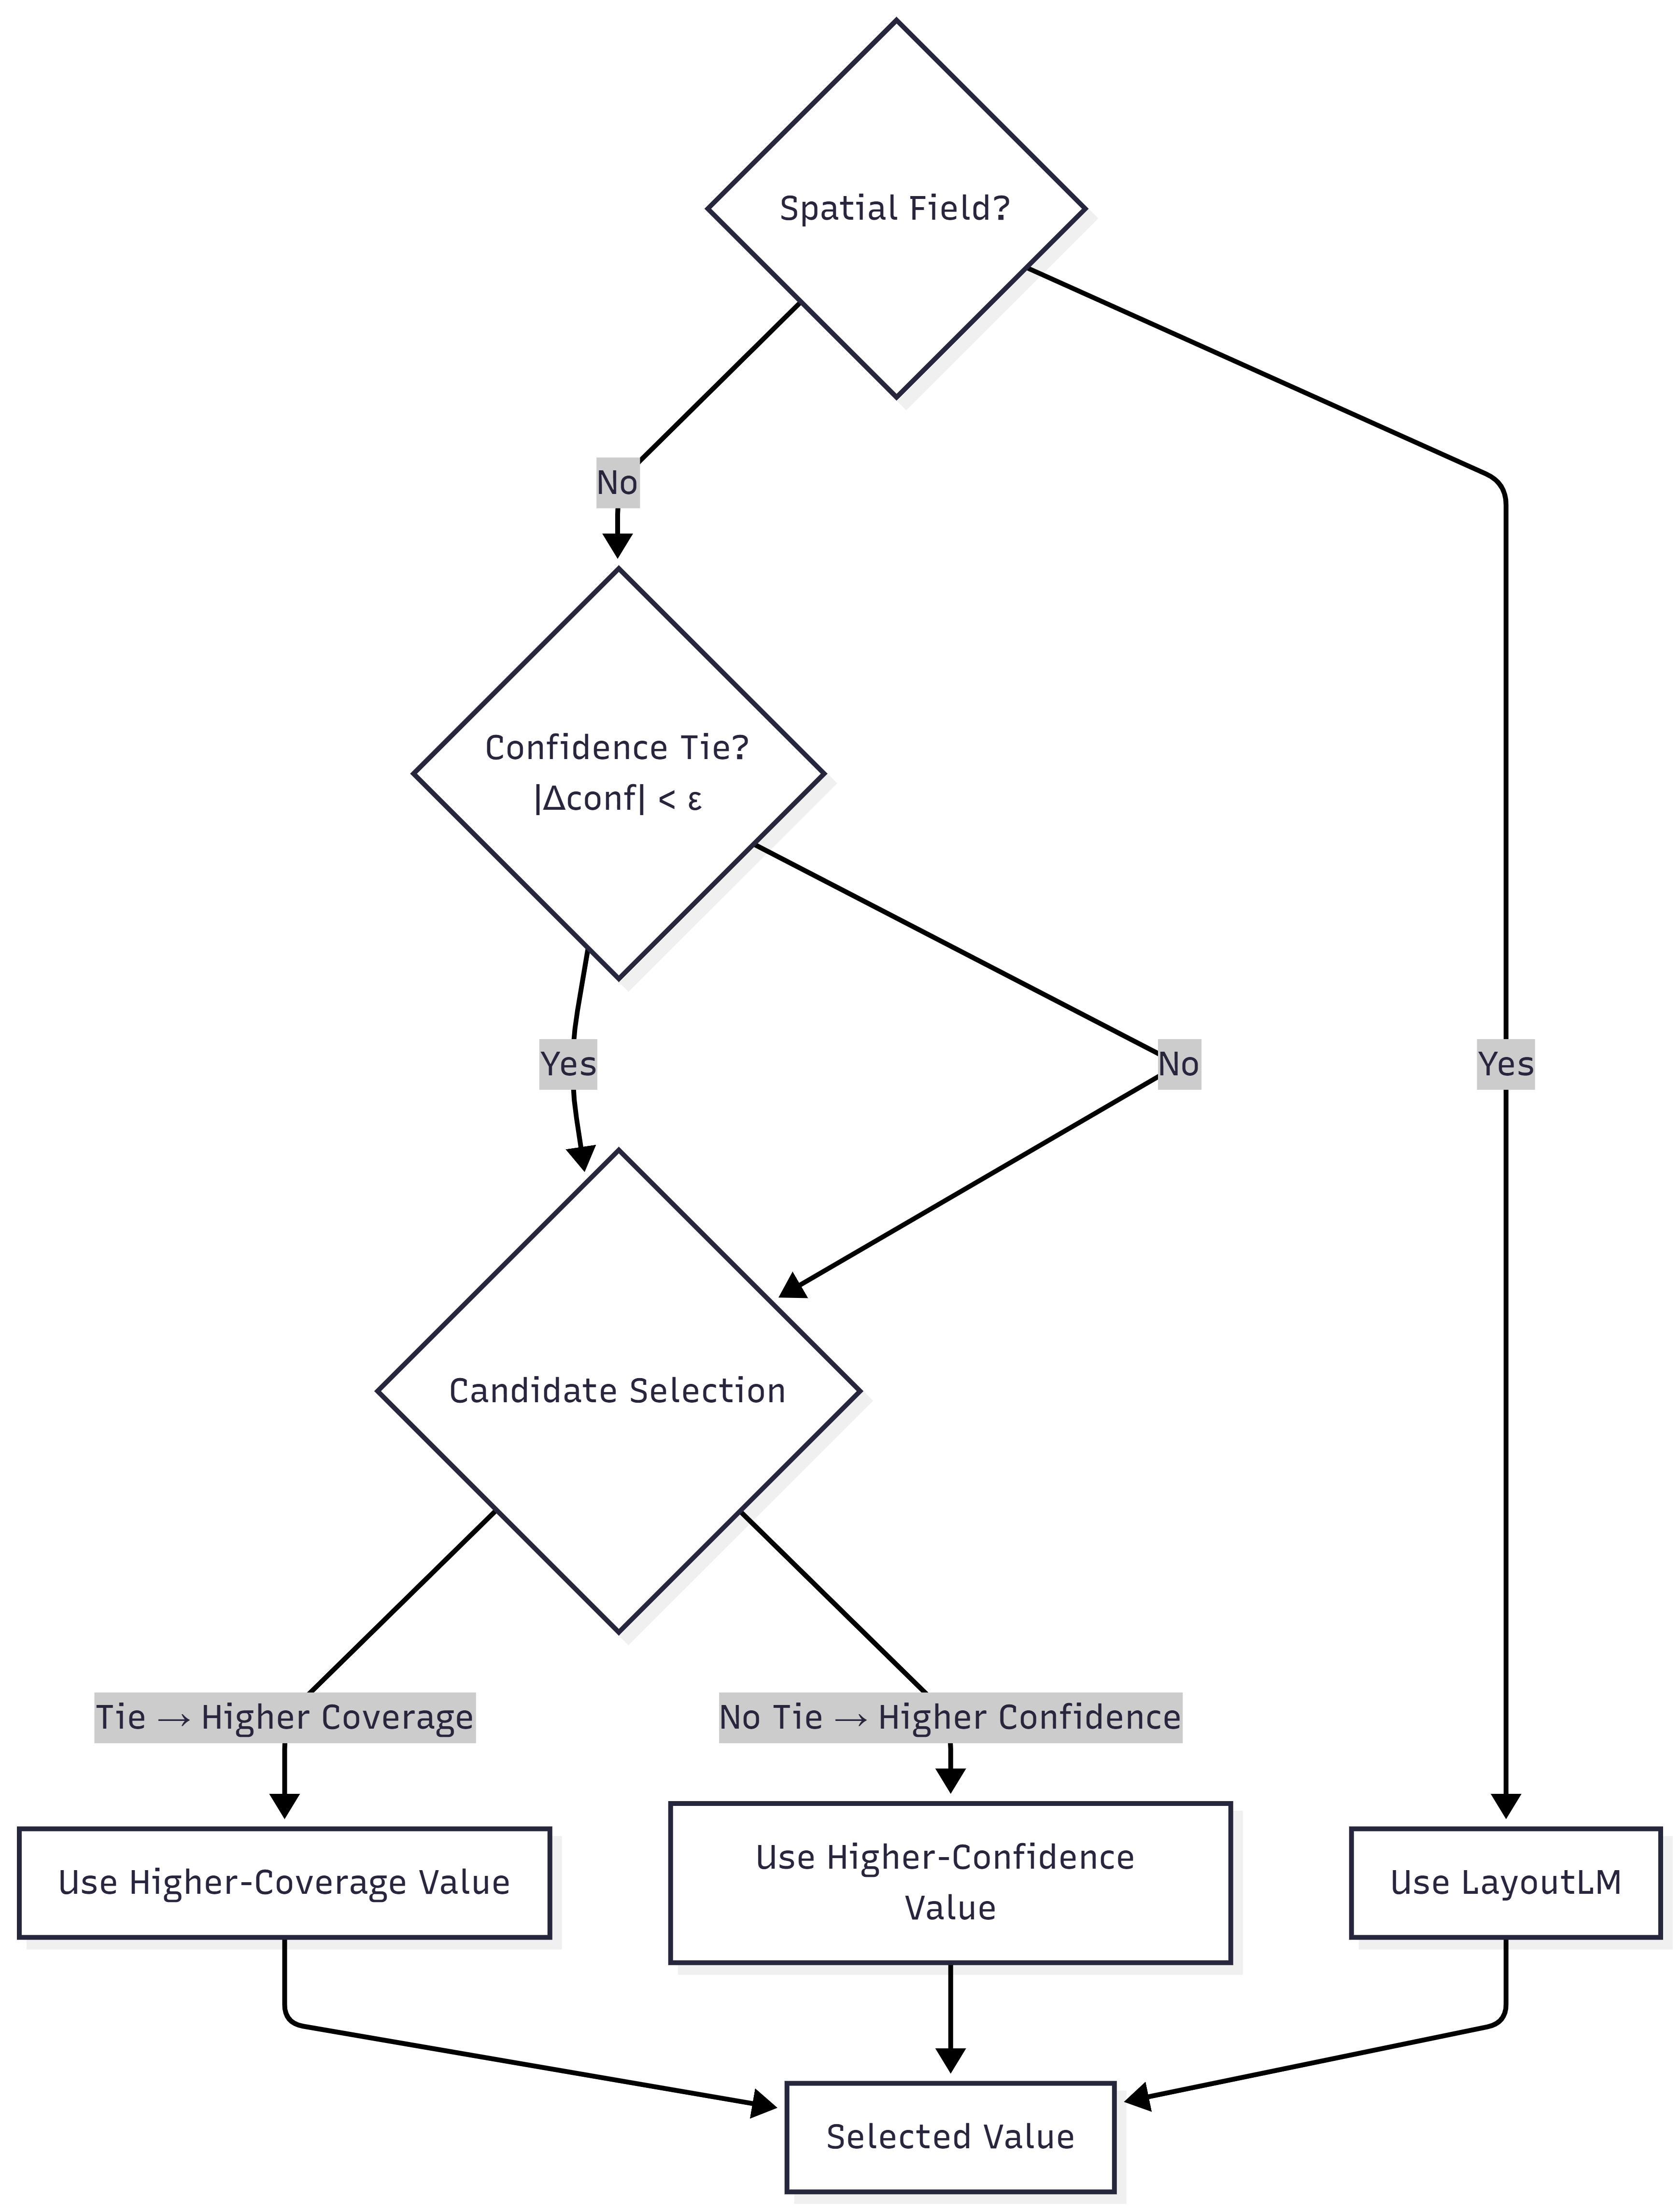
\includegraphics[width=0.75\columnwidth]{parallel_ex.png}
    \caption{Parallel extraction and policy fusion diagram.}
    \label{fig:parallel_extraction}
\end{figure}

We run both Donut and LayoutLM-based extractor on 2 worker threads and output a bundle which includes, for each extractor, a map of field predictions, a confidence map and relevant spatial information.

\subsubsection{Donut OCR-Free Extraction}

 Each field of a schema $f_i$ is extracted by posing a question, composed based on the schema description (like ``What is the invoice date?''), to Donut with the document image. The output consists of:
\begin{equation}
\text{answer}_i = \text{Donut}(\text{image}, q_i)
\end{equation}
The confidence for field $i$ is computed as the average maximum softmax
probability across generated tokens:
\begin{equation}
    c_i^{\text{donut}} = \frac{1}{T} \sum_{t=1}^{T}
    \max_{v} \text{softmax}(s_t)_v
    \label{eq:donut_conf}
\end{equation}
where $s_t$ is the logit vector at generation step $t$ and $T$ is the total
number of generated tokens. Donut's weights are loaded lazily on first use, so
pipelines that never invoke the Donut branch incur no initialization cost.

\subsubsection{Two-Stage FormFiller with Null Handling}

The LayoutLM extraction is based on a two-step procedure. First, a text LLM is given the first 4000 characters of the document together with all field descriptions, resulting in an initial JSON extraction. Second, for any remaining empty field from step 1, we input the field together with the document image to a vision language model in order to infer image- grounded values such as those from a stamp, a table or a signature.

\subsection{Reflexive Policy Fusion}

The policy fusion layer combines both extractor outputs using a set of deterministic rules. By default, fusion doesn't require per-field adjustment except for two fields with very strong spatial correlations (date, money and signature) which are given a field type tag so that they could use the layout to help resolving conflicts for that specific field, all the other fields rely on common signals (availability, confidence, and normalized agreement) only. In case of a conflict with fields with strong spatial correlations, layout predictions from LayoutLM shall be consulted, as the field has a physical location that is close to the label token.
Algorithm~\ref{alg:fusion} summarizes the procedure for a single field.

\begin{algorithmic}[1]
\STATE \textbf{Input:} LayoutLM value $v_L$, confidence $c_L$; Donut value $v_D$, confidence $c_D$; minimum confidence $\delta = 0.15$; agreement tolerance $\epsilon = 0.05$
\IF{$v_L$ is null \AND $v_D$ is null}
    \STATE \textbf{return} null
\ELSIF{exactly one of $v_L, v_D$ is non-null and its confidence $\geq \delta$}
    \STATE \textbf{return} that value
\ELSIF{normalize($v_L$) $=$ normalize($v_D$)}
    \STATE \textbf{return} $v_L$ \COMMENT{LayoutLM value retained for spatial context}
\ELSIF{field is spatially dependent (date, amount, signature)}
    \STATE \textbf{return} $v_L$ \COMMENT{LayoutLM takes precedence on conflict}
\ELSIF{$|c_L - c_D| < \epsilon$}
    \STATE \textbf{return} value with greater coverage of the source region
\ELSE
    \STATE \textbf{return} value with higher confidence
\ENDIF
\end{algorithmic}
\begin{center}
\textit{Algorithm 1: Deterministic field-level policy fusion.}
\end{center}
\label{alg:fusion}

During fusion, normalization is performed, too: a standard technique to filter out common legal jargon, like "as defined herein", removing white spaces and punctuation.

Finally, a cross-field check is done which ensures that dates are consistent (effectivedate $\le$ expirydate), that disclosure and receiving parties are not the same, etc., and marks failed fields.
($\text{effective\_date} \leq \text{expiry\_date}$) and party uniqueness
($\text{disclosing\_party} \neq \text{receiving\_party}$); fields that fail
these checks are flagged with a warning that is propagated into record
metadata rather than being silently corrected.

\subsection{Schema Management, Validation, and Storage}

 The schemas are stored as averaged embeddings (via all-MiniLM-L6-v2) of the field descriptions, and they are fetched using cosine similarity. Schema matching, field normalization, new schema generation in case of a poor match are done by Llama-3.3-70b. The process of record extraction is just checking if the required fields satisfy the type and value constraints.
Invalid fields can be retried or assigned the default value defined by the schema.
All valid records are saved to a SQLITE database.

% -----------------------------------------------------------------------
%  V. EXPERIMENTAL RESULTS AND EVALUATION
% -----------------------------------------------------------------------
\section{Experimental Results and Evaluation}
\label{sec:eval}

\subsection{Experimental Setup}

The LoRA adapters were trained on a Windows~11 workstation with 32\,GB RAM and Python~3.10. We used AdamW as the optimizer with a mini-batch size of 2 and accumulated gradients over 8 steps (total effective batch size of 16). We used FP16 mixed-precision training and trained up to 10 epochs with early stopping on validation macro-F1 score with a patience of 3 epochs.
Standard data augmentation was applied only to the training splits (rotation, brightness/contrast jitter, blur, JPEG compression). The full
configuration is listed in Table~\ref{tab:env}.

\begin{table}[htbp]
\centering
\caption{System Implementation Environment}
\label{tab:env}
\begin{tabular}{ll}
\toprule
\textbf{Component} & \textbf{Configuration} \\
\midrule
OS & Windows~11 / Ubuntu \\
Language & Python~3.10, PyTorch \\
Layout Model & LayoutLMv3-base + LoRA \\
OCR-free Model & Donut-base (naver-clova-ix) \\
LLM (Stage~1) & Llama~3.2 \\
Vision LLM (Stage~2) & Llama~4 Scout (Groq) \\
Schema Agent & Llama-3.3-70b (Groq) \\
OCR & Tesseract \\
Orchestration & LangGraph + LangChain \\
Fine-Tuning & PEFT / LoRA \\
Storage & SQLite (dynamic schema) \\
\bottomrule
\end{tabular}
\end{table}

\subsection{Training Configuration and Results}

Table~\ref{tab:hyperparams} presents the complete settings of both LoRA groups. Cosine learning rate schedule with warmup and layer-wise learning rate decay was adopted. This strategy helped the model to readily adapt to the new datasets while preserving the learned representation from the pre-trained backbone. Both groups training curves can be seen in Fig.~\ref{fig:training_curves}.
The LoRA of Group~1 trained faster, increasing the validation macro-F1 score from 0.5059 in the first epoch to 0.7922 in the eighth epoch, plateauing after epoch 5. Group~1 obtained a validation accuracy of 0.8272 and loss of 0.603 in its best validation run. The LoRA of Group~2 reached the validation macro-F1 score from 0.2489 in the first epoch up to 0.7561 in the sixth epoch and was found to plateaued after epoch 9.
The best validation accuracy for group~2 was 0.8081 and loss 0.605. This is probably caused by heterogeneity on schema and Label sets, which is however not concluded and plateau may result from overfitting in the absence of generalisation test sets. Both group best validation F1 and accuracy are visualised in Fig.~\ref{fig:training_metrics}.

\begin{table}[htbp]
\centering
\caption{Parameter-Efficient Fine-Tuning Configuration}
\label{tab:hyperparams}
\begin{tabular}{ll}
\toprule
\textbf{Configuration Item} & \textbf{Setting} \\
\midrule
Adaptation rank & 16 \\
Scaling coefficient & $2r$ \\
Regularization dropout & 0.05 \\
Adapted transformer layers & Query, Key, Value, Output \\
Mini-batch size & 2 \\
Gradient accumulation & 8 steps \\
Initial learning rate & $3 \times 10^{-4}$ \\
Layer-wise decay factor & 0.9 \\
Learning-rate schedule & Cosine decay + 6\% warmup \\
Maximum training epochs & 10 \\
Early stopping patience & 3 epochs \\
Input sequence length & 512 tokens \\
Numerical precision & FP16 \\
\bottomrule
\end{tabular}
\end{table}

\begin{figure}[htbp]
    \centering
    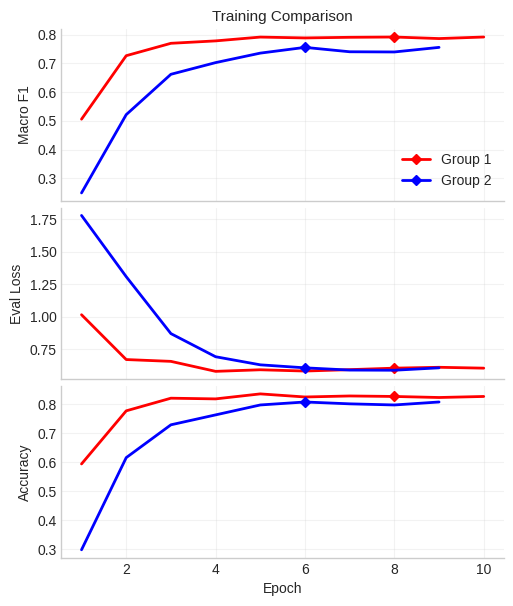
\includegraphics[width=0.65\columnwidth]{training_curves.png}
    \caption{Training comparison of LoRA adapter Groups~1 and~2 across epochs with best performing epochs marked}
    \label{fig:training_curves}
\end{figure}

\begin{figure}[htbp]
    \centering
    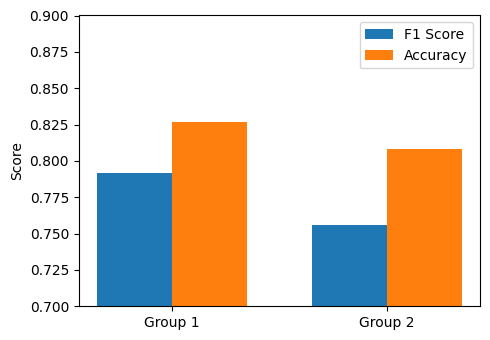
\includegraphics[width=0.6\columnwidth]{training_metrics.png}
    \caption{Best validation F1 score and accuracy achieved by the two LoRA adapter groups.}
    \label{fig:training_metrics}
\end{figure}

\subsection{End-to-End Extraction Performance}

The complete pipeline is evaluated on 15 documents from 5 document categories (invoices, NDAs, employment contracts, land purchase agreements, and instruments of tender for legal tender) over 30 distinct fields. The dataset was purposely generated with various layouts to create challenges for the policy engine. Given its size, the results are more like a proof-of-concept study than a general superiority claim.
The F1 scores in Table~\ref{tab:e2e_aggregate} are calculated at the field level by using the token overlap between predicted and reference values after normalization (i.e., partial-credit F1), instead of the Exact Match Rate also listed in that table; this discrepancy is the reason why Donut can reach high token overlap F1, yet fail to provide an exact match for a large percentage of field values.

\begin{table}[t]
\centering
\caption{Aggregate Extraction Performance Across All Form Types}
\label{tab:e2e_aggregate}
\footnotesize
\setlength{\tabcolsep}{6pt}
\begin{tabular}{lccc}
\toprule
\textbf{Metric} & \textbf{LayoutLM} & \textbf{Donut} & \textbf{Pipeline} \\
\midrule
Avg F1 (token overlap) & 0.904 & 1.000 & \textbf{0.950} \\
Exact Match Rate & \textbf{0.845} & 0.000 & 0.647 \\
Avg Coverage     & 0.845 & 1.000 & \textbf{0.911} \\
Avg Confidence   & 0.582 & 0.802 & 0.722 \\
Avg Latency (s)  & \textbf{4.7}  & 65.6  & 71.8 \\
\bottomrule
\end{tabular}
\end{table}

The two branches each exhibit distinct failure mechanisms. LayoutLM performs exceptionally well in extract spatially referenced fields that directly relate to a specific anchor token, such as for example, NDA party names, or parcel number values from a land deed. On the other hand, it falls short on contexts requiring reasoning across multiple (often non-contingent) regions of the document. As such, LayoutLM coverage does not extend beyond 0.845.

Donut’s decoder scans the entire image document and therefore manages full coverage of all the specified field elements (coverage = 1.000).

However, due to inherent noise during text generation, predicted values from Donut may be “wrapped” in adjacent boilerplate text or content, for example, the extraction of the invoice\_02 document incorrectly identifies an entire repetitive text string such as ``Invoice Date: 2024\ldots'' instead of just the date value. This accounts for Donut’s overall token overlap F1 score of 1.000 alongside its Exact Match Rate of 0.000. The policy layer leverages general, field-invariant signals for the majority of the document elements, with field type-specific spatial reasoning to handle elements that rely on a unique location.

By integrating Donut’s complete coverage to compensate for LayoutLM’s deficiencies, and favouring LayoutLM’s high-precision for conflicts stemming from spatial references, the post-fusion normalization mechanism rectifies errors and ‘cleans up’ boilerplate surrounding Donut’s output, enabling a coverage of 0.911 and mean confidence of 0.722 (falling between the two components but never surpassing both), token overlap F1 of 0.950 (not reaching the Donut level of 1.000, but superior to LayoutLM’s 0.904), and an Exact Match Rate of 0.647 (drastically outperforming Donut's 0.000). Though the pipeline may not triumph on every single metric, it considerably enhances reliability for exact matches when compared to Donut, while effectively maintaining LayoutLM’s accuracy and Donut’s coverage. The total pipeline extraction process took 71.8s.
This is an increase over the slower single branch (Donut took 65.6s) by 6.2s.

As all processing within the two branches occurred in parallel, the effective wall-clock time is the time spent in the longer branch plus the processing time outside of this parallel phase (synchronization, policy decision, normalization, and validation). This indicates that the 6.2s overhead is solely for the serial processing, not the parallel component.

\subsection{Adapter Storage Efficiency}

Each of the LoRA adapters has a storage cost of around $12\,\text{MB}$, compared to around $500\,\text{MB}$ for a fully fine-tuned LayoutLMv3 checkpoint. Loading and switching groups of adapters cost less than $200\,\text{ms}$.

\subsection{Schema Registry Retrieval}

\begin{figure}[htbp]
    \centering
    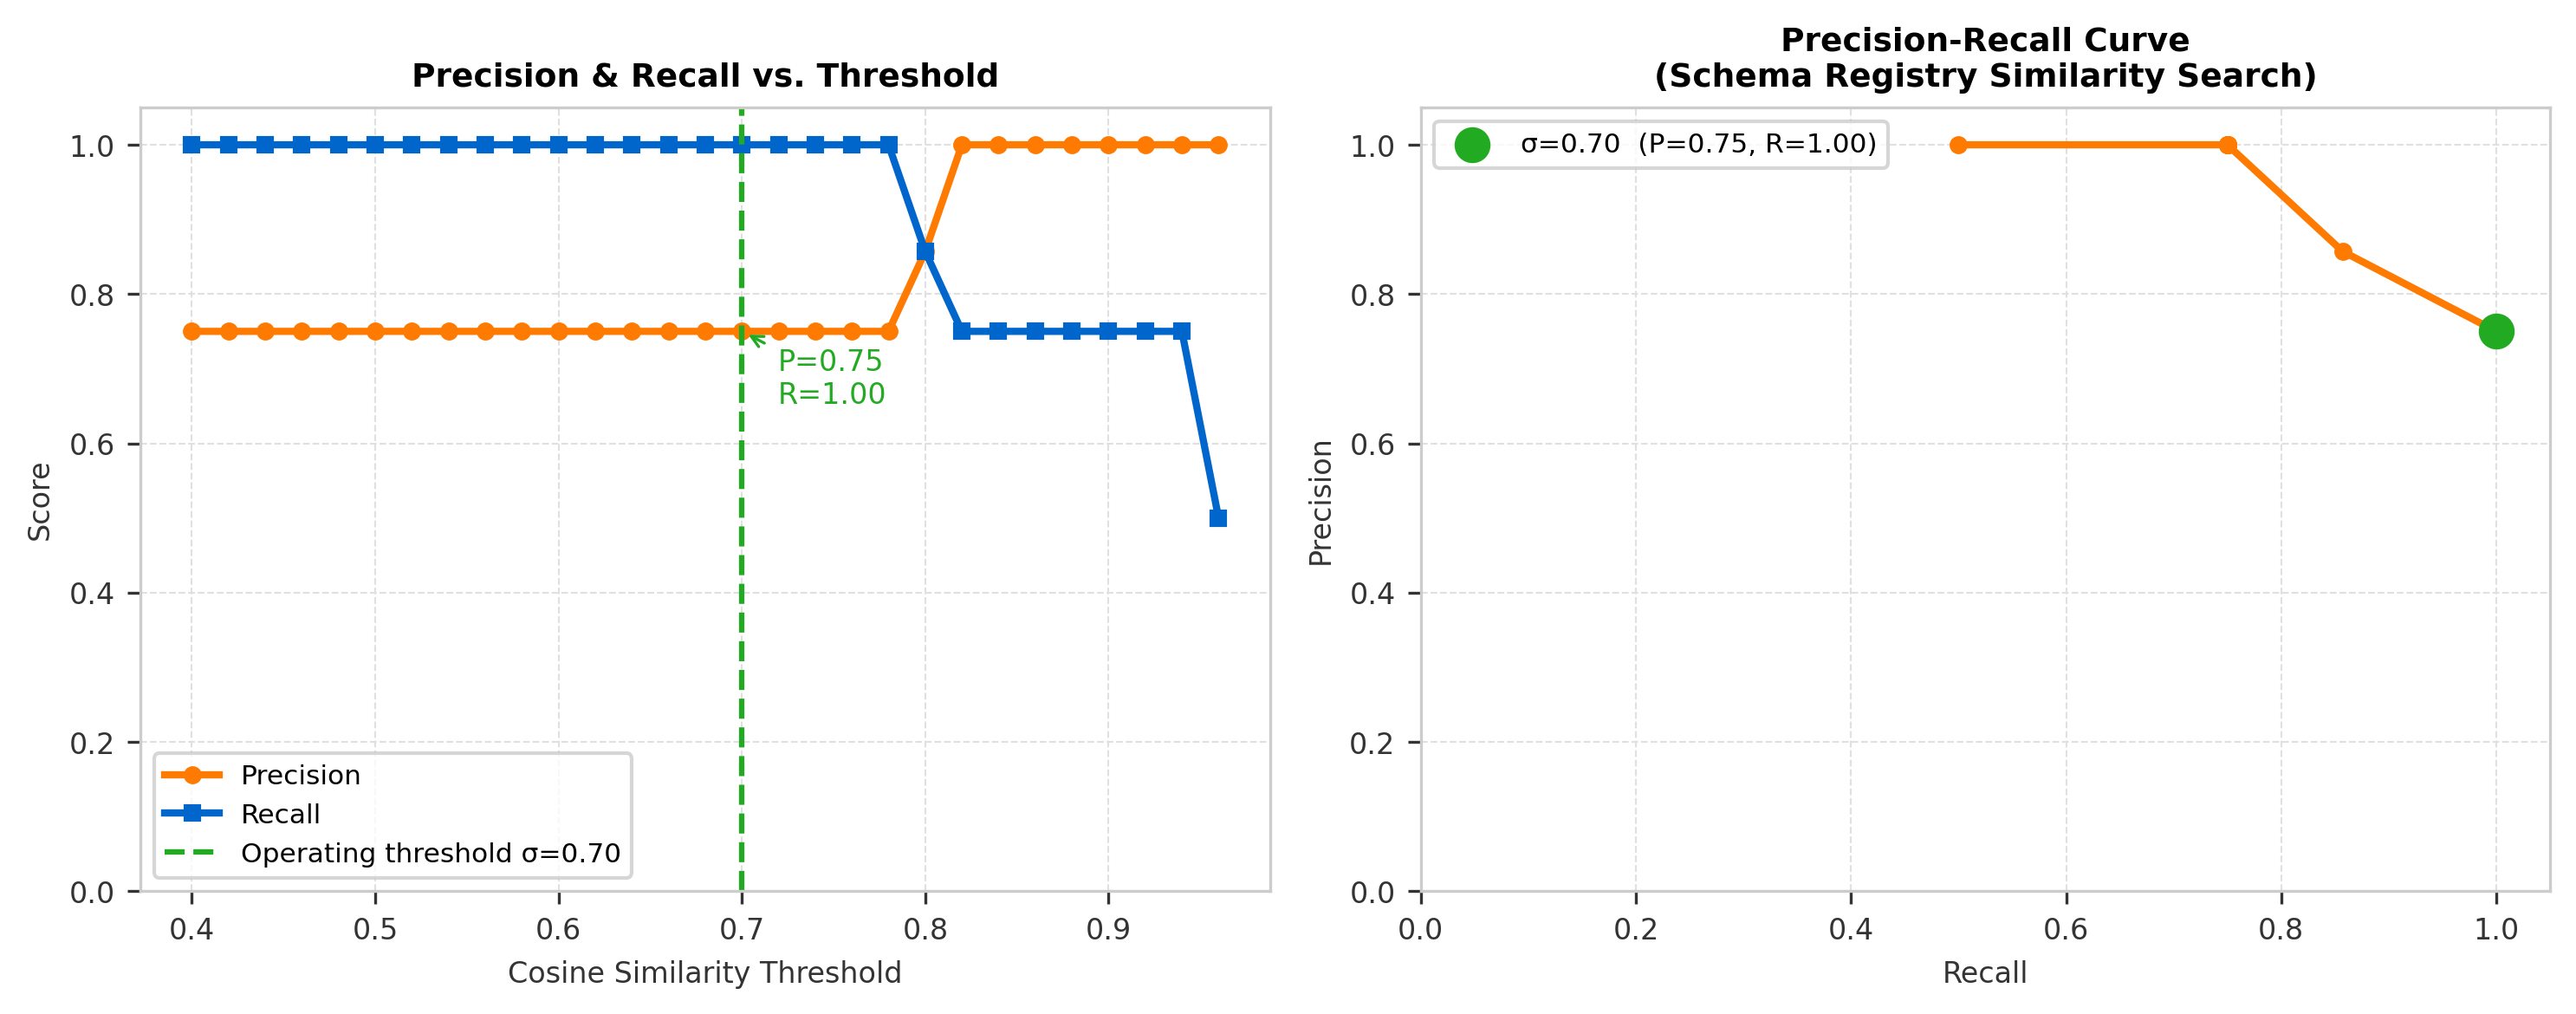
\includegraphics[width=\columnwidth]{schema_registry.png}
    \caption{Precision--recall trade-off for schema registry similarity search
    at differing cosine similarity thresholds}
    \label{fig:schema_pr_curve}
\end{figure}

Figure \ref{fig:schema_pr_curve} presents the precision-recall trade-off for the registry retrieval stage when the cosine similarity threshold varies from 0.40 to 0.96, with registry retrieval evaluated on schema queries originating from 15 end-to-end documents into a registry created using the schema information of five core document types. Higher thresholds produce fewer candidates but improve precision, while lower thresholds lead to increased recall at the expense of precision. We set $\sigma=0.70$ as the default operating threshold in section \ref{sec:arch}, and here we have chosen $\sigma=0.80$ from our preliminary evaluation in which this threshold provides a well-balanced precision-recall score (0.857, 0.857) over the evaluated queries. 

% -----------------------------------------------------------------------
%  VI. CONCLUSION
% -----------------------------------------------------------------------
\section{Conclusion}
\label{sec:conclusion}

This paper proposes a policy-guided, schema-aware approach to semi-structured document information extraction. This approach integrates layout-aware and OCR-free models, with a schema-guided, deterministic fusion method, schema retrieval, validation, and parameter-efficient fine-tuning with LoRA adapters. The LoRA adapters obtained a validation macro-F1 of 0.7922 and 0.7561 with 12 MB per adapter of storage. Our proof-of-concept pipeline achieved a token-overlap F1 of 0.950 and coverage of 0.911 on this small-scale benchmark. While 15 documents prevent robust conclusion of performance and broad generalizability, these promising results demonstrate the viability of our policy-guided, schema-aware framework for information extraction from semi-structured documents. Our next step is to conduct evaluations on large benchmark datasets, include standard external baseline systems, run multiple trials of the experiments, and conduct a component-wise ablation study to better understand the contributions of individual components.

% -----------------------------------------------------------------------
%  VII. FUTURE WORK
% -----------------------------------------------------------------------
\section{Future Work}
\label{sec:future}

Future directions involve implementing more domain-specific LoRA adapters for richer routing capabilities, unifying extraction to a single multimodal LLM in place of current extractors to enhance recall for challenging fields, broadening the capabilities to multilingual documents by augmenting with other adapters trained over resources such as XFUND and CORD \cite{park2019cord} and introducing a graph-based table detector \cite{yu2021pick} for table content extraction.

% -----------------------------------------------------------------------
%  REFERENCES
% -----------------------------------------------------------------------

\begin{thebibliography}{99}

\bibitem{publaynet}
X.~Zhong, J.~Tang, and A.~Jimeno-Yepes,
``PubLayNet: Largest dataset ever for document layout analysis,''
in \textit{Proc. International Conference on Document Analysis and
Recognition (ICDAR)}, 2019, pp.~1015--1022.

\bibitem{binmakhashen2020}
G.~M.~Binmakhashen and S.~A.~Mahmoud,
``Document layout analysis: A comprehensive survey,''
\textit{ACM Computing Surveys}, vol.~52, no.~6,
Art.~109, pp.~1--36, 2020.

\bibitem{docbank}
M.~Li, Y.~Xu, L.~Cui, S.~Huang, F.~Wei, Z.~Li, and M.~Zhou,
``DocBank: A benchmark dataset for document layout analysis,''
in \textit{Proc. 28th International Conference on Computational
Linguistics (COLING)}, 2020, pp.~949--960.

\bibitem{lee2022formnet}
C.-Y.~Lee, C.-L.~Li, T.~Dozat, V.~Perot, G.~Su, N.~Hua,
J.~Ainslie, R.~Wang, Y.~Fujii, and T.~Pfister,
``FormNet: Structural encoding beyond sequential modeling in form
document information extraction,''
in \textit{Proc. 60th Annual Meeting of the Association for
Computational Linguistics (ACL)}, 2022, pp.~3735--3754.

\bibitem{kim2022donut}
G.~Kim, T.~Hong, M.~Yim, J.~Nam, J.~Park, J.~Yim,
W.~Hwang, S.~Yun, D.~Han, and S.~Park,
``OCR-free document understanding transformer,''
in \textit{Proc. European Conference on Computer Vision (ECCV)},
2022, pp.~498--517.

\bibitem{layoutlm}
Y.~Xu, M.~Li, L.~Cui, S.~Huang, F.~Wei, and M.~Zhou,
``LayoutLM: Pre-training of text and layout for document image
understanding,''
in \textit{Proc. 26th ACM SIGKDD International Conference on
Knowledge Discovery and Data Mining (KDD)}, 2020,
pp.~1192--1200.

\bibitem{layoutlmv2}
Y.~Xu, Y.~Xu, T.~Lv, L.~Cui, F.~Wei, G.~Wang, Y.~Lu,
D.~Florencio, C.~Zhang, W.~Che, M.~Zhang, and L.~Zhou,
``LayoutLMv2: Multi-modal pre-training for visually-rich document
understanding,''
in \textit{Proc. 59th Annual Meeting of the Association for
Computational Linguistics and the 11th International Joint Conference
on Natural Language Processing (ACL-IJCNLP)}, 2021,
pp.~2579--2591.

\bibitem{layoutlmv3}
Y.~Huang, T.~Lv, L.~Cui, Y.~Lu, and F.~Wei,
``LayoutLMv3: Pre-training for document AI with unified text and
image masking,''
in \textit{Proc. 30th ACM International Conference on Multimedia
(ACM MM)}, 2022, pp.~4083--4091.

\bibitem{react2023}
S.~Yao, J.~Zhao, D.~Yu, N.~Du, I.~Shafran, K.~Narasimhan,
and Y.~Cao,
``ReAct: Synergizing reasoning and acting in language models,''
in \textit{Proc. International Conference on Learning
Representations (ICLR)}, 2023.

\bibitem{reflexion2023}
N.~Shinn, F.~Cassano, A.~Gopinath, K.~Narasimhan, and S.~Yao,
``Reflexion: Language agents with verbal reinforcement learning,''
in \textit{Advances in Neural Information Processing Systems},
vol.~36, 2023, pp.~8634--8652.

\bibitem{selfrefine2023}
A.~Madaan, N.~Tandon, P.~Gupta, S.~Hallinan, L.~Gao,
S.~Wiegreffe, U.~Alon, N.~Dziri, S.~Prabhumoye,
Y.~Yang, S.~Gupta, B.~P.~Majumder, K.~Hermann,
S.~Welleck, A.~Yazdanbakhsh, and P.~Clark,
``Self-Refine: Iterative refinement with self-feedback,''
in \textit{Advances in Neural Information Processing Systems},
vol.~36, 2023, pp.~46534--46594.

\bibitem{gptner2024}
S.~Wang, X.~Sun, X.~Li, R.~Ouyang, F.~Wu, T.~Zhang,
J.~Li, and G.~Wang,
``GPT-NER: Named entity recognition via large language models,''
in \textit{Findings of the Association for Computational Linguistics:
NAACL 2024}, 2024, pp.~4488--4503.

\bibitem{instructor2023}
H.~Su, J.~Kasai, C.~H.~Wu, W.~Shi, T.~Wang,
J.~Xin, R.~Zhang, M.~Ostendorf, L.~Zettlemoyer,
N.~A.~Smith, and T.~Yu,
``One Embedder, Any Task: Instruction-finetuned text embeddings,''
in \textit{Findings of the Association for Computational Linguistics:
ACL 2023}, 2023, pp.~1102--1121.

\bibitem{guidance2023}
S.~Willard and R.~Louf,
``Efficient guided generation for large language models,''
\textit{arXiv preprint arXiv:2307.09702}, 2023.

\bibitem{ji2023hallucination}
Z.~Ji, N.~Lee, R.~Frieske, T.~Yu, D.~Su, Y.~Xu,
E.~Ishii, Y.~J.~Bang, A.~Madotto, and P.~Fung,
``Survey of hallucination in natural language generation,''
\textit{ACM Computing Surveys}, vol.~55, no.~12,
Art.~248, pp.~1--38, 2023.

\bibitem{hu2022lora}
E.~J.~Hu, Y.~Shen, P.~Wallis, Z.~Allen-Zhu, Y.~Li,
S.~Wang, L.~Wang, and W.~Chen,
``LoRA: Low-rank adaptation of large language models,''
in \textit{Proc. International Conference on Learning
Representations (ICLR)}, 2022.

\bibitem{cuad2021}
D.~Hendrycks, C.~Burns, A.~Chen, and S.~Ball,
``CUAD: An expert-annotated NLP dataset for legal contract review,''
in \textit{Advances in Neural Information Processing Systems},
vol.~34, 2021, pp.~13836--13849.

\bibitem{yu2021pick}
W.~Yu, N.~Lu, X.~Qi, P.~Gong, and R.~Xiao,
``PICK: Processing key information extraction from documents using
improved graph learning-convolutional networks,''
in \textit{Proc. 25th International Conference on Pattern Recognition
(ICPR)}, 2021, pp.~4363--4370.

\bibitem{luo2023geolayoutlm}
C.~Luo, C.~Cheng, Q.~Zheng, and C.~Yao,
``GeoLayoutLM: Geometric pre-training for visual information extraction,''
in \textit{Proc. IEEE/CVF Conference on Computer Vision and Pattern
Recognition (CVPR)}, 2023, pp.~7092--7101.

\bibitem{hwang2021cost}
W.~Hwang, H.~Lee, J.~Yim, G.~Kim, and M.~Seo,
``Cost-effective end-to-end information extraction for
semi-structured document images,''
in \textit{Proc. 2021 Conference on Empirical Methods in Natural
Language Processing (EMNLP)}, 2021, pp.~3375--3383.

\bibitem{davis2022dessurt}
B.~Davis, B.~Morse, B.~Price, C.~Tensmeyer,
C.~Wigington, and V.~Morariu,
``End-to-end document recognition and understanding with Dessurt,''
\textit{arXiv preprint arXiv:2203.16618}, 2022.

\bibitem{mathew2021docvqa}
M.~Mathew, D.~Karatzas, and C.~V.~Jawahar,
``DocVQA: A dataset for VQA on document images,''
in \textit{Proc. IEEE Winter Conference on Applications of Computer
Vision (WACV)}, 2021, pp.~2200--2209.

\bibitem{he2022unified}
J.~He, C.~Zhou, X.~Ma, T.~Berg-Kirkpatrick, and G.~Neubig,
``Towards a unified view of parameter-efficient transfer learning,''
in \textit{Proc. International Conference on Learning
Representations (ICLR)}, 2022.

\bibitem{jaume2019funsd}
G.~Jaume, H.~K.~Ekenel, and J.-P.~Thiran,
``FUNSD: A dataset for form understanding in noisy scanned
documents,''
in \textit{Proc. ICDAR Workshops}, 2019, pp.~1--6.

\bibitem{park2019cord}
S.~Park, S.~Shin, B.~Lee, J.~Lee, J.~Surh, M.~Seo, and H.~Lee,
``CORD: A consolidated receipt dataset for post-OCR parsing,''
in \textit{NeurIPS 2019 Workshop on Document Intelligence}, 2019.

\end{thebibliography}

\end{document}